\begin{frame}
	\centering
	\fontsize{22pt}{24pt}\selectfont
	Capacidade Absortiva e Aprendizagem Organizacional
\end{frame}

\begin{frame}{Referências}
    \begin{vfilleditems}
    \footnotesize
    \item \fullcite{cohen1990absorptive} (\textcolor{red}{Empírico, seminal e com uma boa amostragem})
    \item \fullcite{zahra2002absorptive} (\textcolor{red}{Conceitual, seminal})
    \item \fullcite{staples2001opportunities} (\textcolor{red}{Conceitual, seminal})
    \end{vfilleditems}
\end{frame}

\begin{frame}{Capacidade Absortiva}
	\Large A capacidade de uma organização de reconhecer o valor
	de informações novas e externas, assimilá-las e aplicá-las
	\parencite{cohen1990absorptive}.
\end{frame}

\begin{frame}{Modelo de Capacidade Absortiva e Incentivos de P\&D}
	\begin{figure}
		\centering
		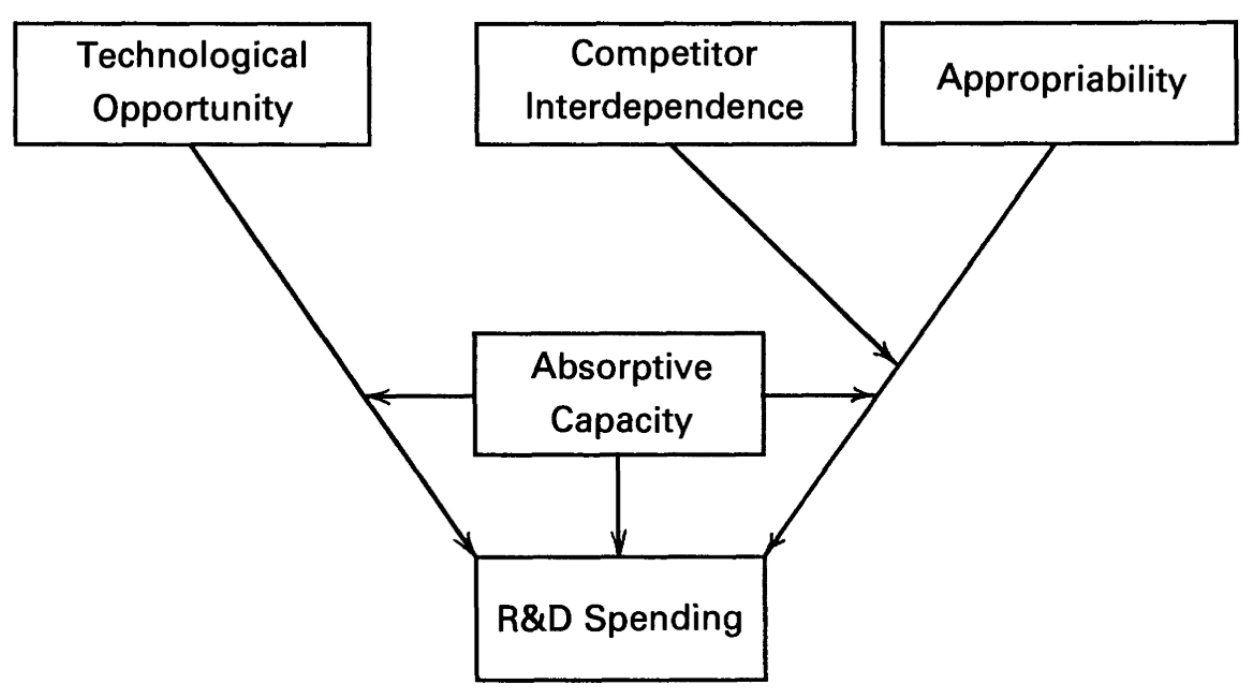
\includegraphics[width=0.75\textwidth]{absorptive_capacity.png}
		\caption{Fonte: \textcite{cohen1990absorptive}.}
		\label{fig:absorptive_capacity}
	\end{figure}
\end{frame}

\begin{frame}{Modelo de Fontes de Conhecimento Tecnológico Organizacional}
	\begin{figure}
		\centering
		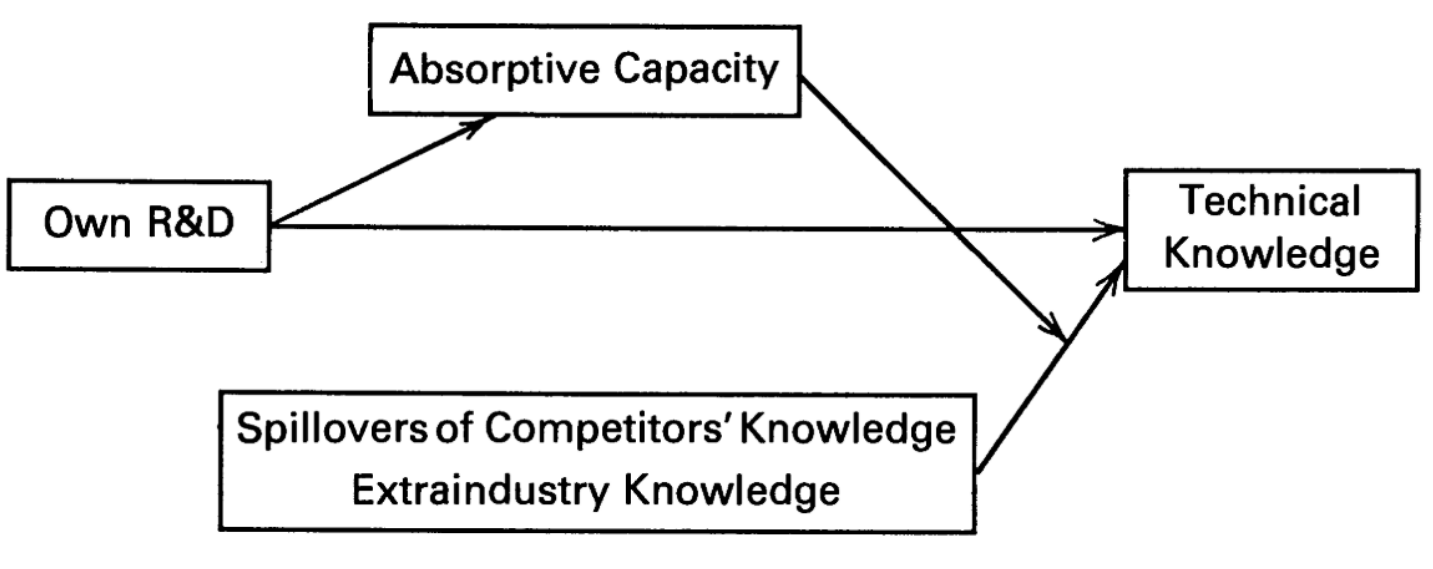
\includegraphics[width=0.85\textwidth]{absorptive_capacity2.png}
		\caption{Fonte: \textcite{cohen1990absorptive}.}
		\label{fig:absorptive_capacity2}
	\end{figure}
\end{frame}

\begin{frame}{Mensurações de \textcite{cohen1990absorptive}}
	\textbf{Dependente}: Intensidade de P\&D (em \% de vendas)
	\vfill
	\textbf{Independentes}:
	\begin{vfilleditems}
	\item Oportunidade Tecnológica - Likert 7-pontos
		\begin{vfilleditems}
		\item \textcolor{green}{Base Científica do Setor}
		\item Fontes de Conhecimento Extrasetor:
			\begin{vfilleditems}
			\item \textcolor{red}{Fornecedores de equipamentos}
			\item \textcolor{red}{Fornecedores de materiais}
			\item \textcolor{green}{Usuários dos Produtos do Setor}
			\item \textcolor{green}{Laboratórios e Agências Governamentais}
			\item \textcolor{green}{Universidades}
			\end{vfilleditems}
		\end{vfilleditems}
	\item Apropriabilidade: Intensidade que as empresas protegem a vantagem competitiva de novos produtos (Patentes etc.)
	\end{vfilleditems}
\end{frame}

\begin{frame}{Modelo de Capacidade Absortiva}
	\begin{figure}
		\centering
		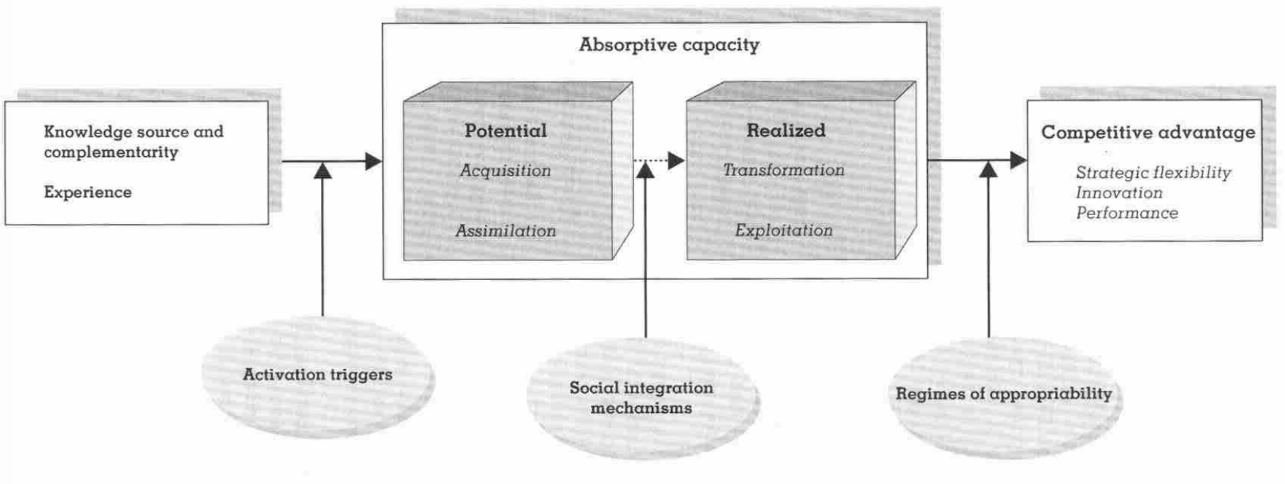
\includegraphics[width=1.0\textwidth]{absorptive_capacity3.png}
		\caption{Fonte: \textcite{zahra2002absorptive}.}
		\label{fig:absorptive_capacity3}
	\end{figure}
\end{frame}

\begin{frame}{Modelo de Visão Baseada em Conhecimento}
	\begin{figure}
		\centering
		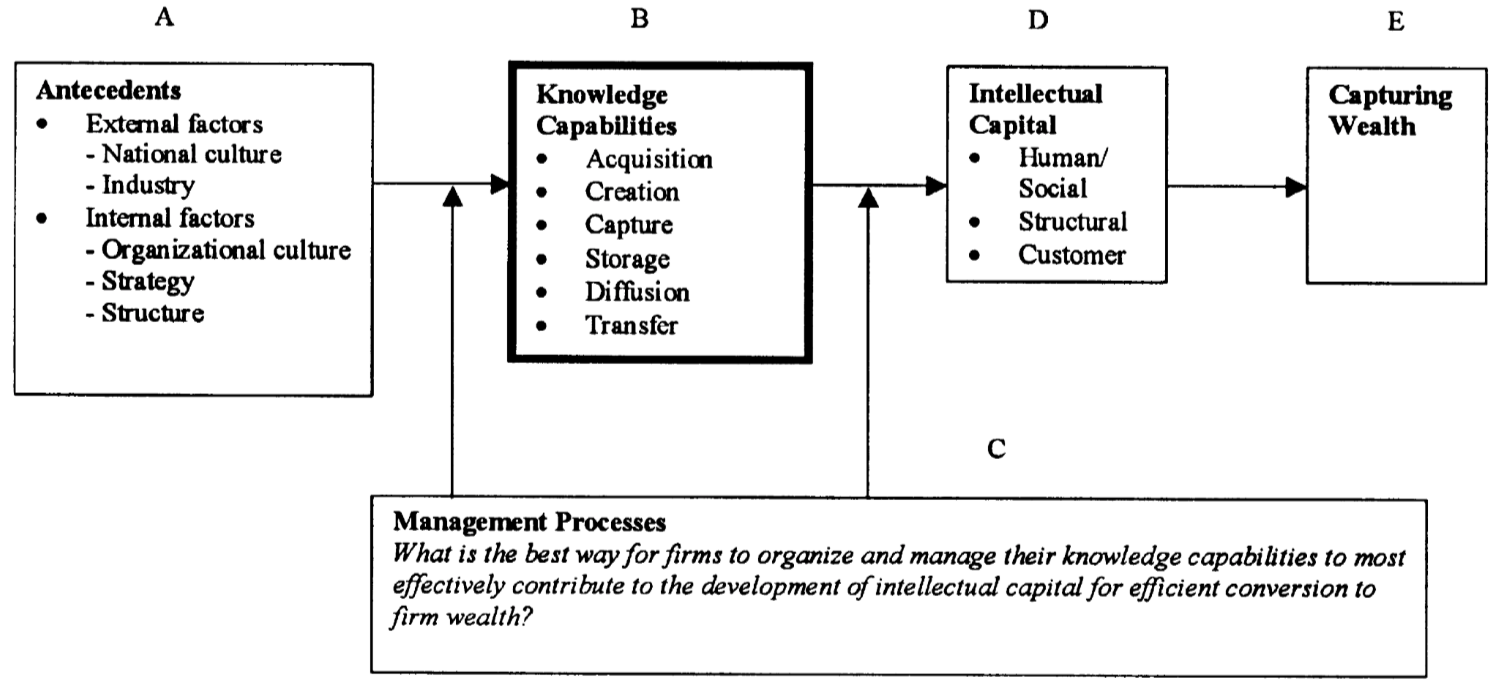
\includegraphics[width=0.85\textwidth]{kbv.png}
		\caption{Fonte: \textcite{staples2001opportunities}.}
		\label{fig:kbv}
	\end{figure}
\end{frame}
